\documentclass[twocolumn]{aastex62}
\usepackage{natbib}
\usepackage[colorinlistoftodos]{todonotes}
%\usepackage{academicons}
%\definecolor{orcidlogocol}{HTML}{A6CE39}
\bibliographystyle{apj}

\begin{document}

\title{COLLISION RATES OF PLANETESIMALS NEAR MEAN-MOTION RESONANCES}

\author{Spencer C. Wallace}
\affiliation{Astronomy Department, University of Washington, Seattle, WA 98195}

\author{Aaron C. Boley}
\affiliation{Department of Physics and Astronomy, University of British Columbia, Vancouver BC, Canada}

\author{Thomas R. Quinn}
\affiliation{Astronomy Department, University of Washington, Seattle, WA 98195}

\begin{abstract}
A perturbing planet can leave a lasting imprint a debris disk near the locations of mean motion resonances (MMRs). Unfortunately, the planetesimal-sized objects that make up the majority of these disks are extremely difficult to directly observe. Dust created from collisions between planetesimals may be a much better way to constrain the structure of these disks. We use a direct N-body model to measure planetesimal collision rates in a dynamically cold debris disk composed of 150 km bodies. Even though the eccentricities are pumped at the nominal resonance locations, conservation of the Jacobi energy pushes planetesimals inward and enhances the collision rate adjacent to the resonances. In addition, we find that the collision rate is severely throttled near the 3:1 MMR and that a tightly wound spiral wave is launched from this location.
\end{abstract}

\section{Introduction} \label{sec:intro}

Recent observations of circumstellar disks by ALMA have revealed a rich variety of substructure in the millimeter wavelength contiunuum emission. Features such as gaps and asymmetries \citep{2015ApJ...808L...3A, 2016Sci...353.1519P, PhysRevLett.117.251101, 2016ApJ...820L..40A, 2016Natur.535..258C} in the emission provide diagnostics for the physical processes that drive the evolution of the disks. At these wavelengths, much of this light is produced by second-generation debris generated through collisional grinding of planetesimals \citep[see][]{2008ARA&A..46..339W}. 

In some cases, these gap features are argued to be an indicator for the presence of a giant planet, either embedded in the disk \citep{2015MNRAS.453L..73D} or orbiting externally. An giant perturber can influence the structure of the dust emission in a number of ways. A misaligned giant planet can produce nonaxisymmetric features such as warps \citep{2001A&A...370..447A}. Highly eccentric perturbers can produce even more complicated structures through secular perturbations \citep{2014MNRAS.443.2541P, 2015MNRAS.448.3679P}. Mean motion resonances (MMRs) have been shown to open gaps as well \citep{2015ApJ...798...83N, 2016ApJ...818..159T, 2018ApJ...857....3T}.

The dynamics governing the motion of bodies near MMRs is extremely nonlinear, as is determining what the collision rates between planetesimals should look like in these regions. For a collection of bodies massive enough to experience the effects of gravitational focusing, a large eccentricity dispersion tends to reduce the probability of collision, while enhancements in surface density tends to increase it. Due to conservation of the Jacobi energy, MMRs simultaneously enhance the local eccentricity dispersion and also enhance the surface density adjacent to the resonance \citep{2000Icar..143...45R, 2017ApJ...850..103B}.

Because the second generation dust production is driven by the planetesimal collision rate, it is crucial to understand how the dynamics that drive collisions works. In particular, it is not obvious how to link the readily observable thermal emission from dust in protoplanetary disks to the presence of a perturbing giant planet. Due to its nonlinearity, this problem is best studied with N-body simulations. Unfortunately, collision detection in an N-body simulation is extremely computationally expensive. So far, studies of planetesimal dynamics near MMRs have involved either collisionless test particles \citep{2017ApJ...850..103B, 2016ApJ...818..159T, 2018ApJ...857....3T} or severely limited integration times \citep{2000Icar..143...45R}.

To further elucidate this subject, we use the tree based N-body code {\sc ChaNGa} \citep{2008IEEEpds...ChaNGa, 2015AphCom..2..1} to follow the collisional evolution of a planetesimal disk under the gravitational influence of a Jupiter sized body. Because particle positions are sorted into a tree structure, neighbor finding and collision detection can be done quickly and efficiently. This considerably relaxes the constraints on resolution and integration time. With this toolset, we explore the collision rate structure of the planetesimal disk in the vicinity of mean motion resonances.

This work is organized in the following way. In section \ref{sec:dynamics} we provide an overview of the dynamics that drive the evolution of a planetesimal disk under the gravitational influence of an external perturber. In section \ref{sec:setup} we describe the N-body code we use and describe how we constructed the initial conditions for the two simulations that are run: one with a perturber on a circular orbit and one with an eccentric perturber. Section \ref{sec:results} goes on to explore the results of the two, with particular focus on the radial variation in the collision rates. In section \ref{sec:dust}, we use the positions of the collision events to construct a map of second generation dust emission, under the assumption that dust grains produced by collisions will immediately couple to the gas and circularize their orbits. Finally, we assess the observability of features in the dust emission due to mean motion resonances and conclude in section \ref{sec:discuss}.

\section{Collisions and Mean Motion Resonances} \label{sec:dynamics}

\section{Simulation Setup} \label{sec:setup}

We use equation 12 from kokubo and ida 2002 to set initial free eccentricites and inclinations for particles, in equilibrium with gas drag. These would be about twice as big if we instead used vrandom = vesc, which is the point at which grav stirring stops being very effective. Forced eccentricity and varpi set by secular perturbations by Jupiter, as done by Tabeshian and Weigert.

\section{Results} \label{sec:results}

\section{Dust Emission} \label{sec:results}

\section{Summary and Discussion} \label{sec:discuss}

\begin{figure}
    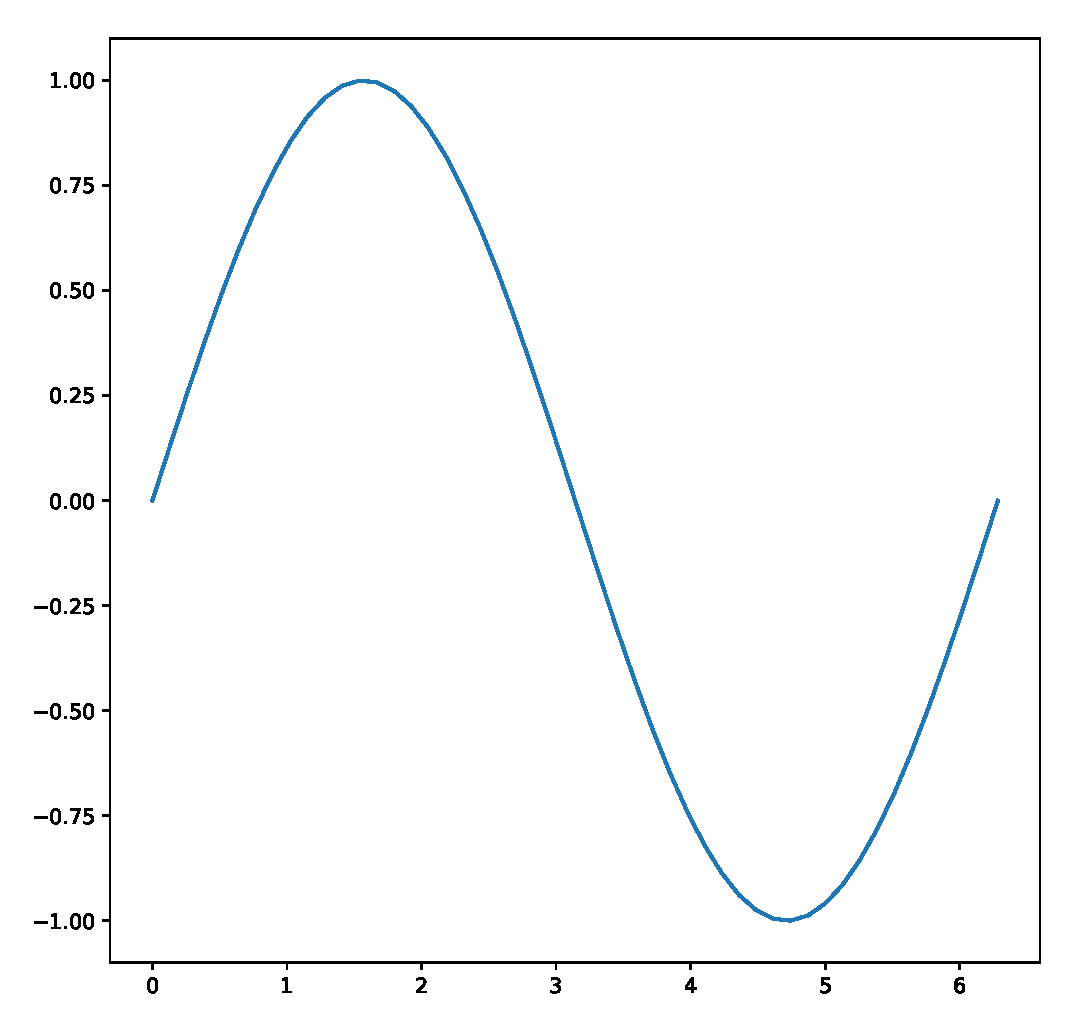
\includegraphics[width=\columnwidth]{figures/test.eps}
    \caption{Caption goes here.
    \label{fig:test}}
\end{figure}

%In this study, we will consider the effects that an external perturber has on the dynamical evolution and collision rates of planetesimals in a circumstellar disk. Planetesimals are too small to reflect much star light and are of too low mass to have any significant amount of thermal inertial. However, the large amounts of dust produced by collisional grinding can be used to infer where planetesimals are interacting \citep{2005Natur.436..363S, 2015ApJ...806...23L}. Although the behavior of the small dust grains can strongly depend on the hydrodynamic behavior of the gas \citep{2015ApJ...813L..14B}, the evolution of the planetesimals (km sized and larger) should be well decoupled from the gas. This means that results of this study should be applicable to both gas rich protoplanetary disks such as HL Tau and TW Hya, along with dusty debris disks such as Fomalhut \citep{2017ApJ...842....8M}.

%The intermediate stages of planet formation are incredibly difficult to observe. Planetesimals, which are the building blocks of planets, are too small to reflect any significant amount of star light and are of too low mass to carry much thermal inertia. However, large volumes of dust produced through collisional grinding of planetesimals can be used to infer where planetesimals are interacting 

%In the Solar System, the formation of Jupiter is thought to have destabilized the orbits of nearby planetesimals and triggered a short and intense period of bombardment. In addition to triggering a cascade of collisional grinding \citep{2012ApJ...750....8T}, the formation of Jupiter is thought to have facilitated the mixing of volatiles in the inner Solar System \citep{2017Icar..297..134R}.

%From an outsider's perspective, the most easily observable property of the Solar System is the infrared emission from small dust grains. Outside the Solar System, infrared excess has also been tied to the presence of dust (citation needed). Recent high resolution images from ALMA have shown that the structure of these dusty disks around other stars can have rather complicated structures.

%Talk about observed gaps in ALMA images of PPDs. Many different explanations for rings and gaps \citep{2019arXiv190103680V}. One possible explanation is resonances with outer companion. \citet{2017ApJ...850..103B} examined this possibility, but used massless test particles to represent the planetesimals. Although this provided some information about how the planetesimals move under the influence of a mean motion resonance, it did not say anything about where the collisions and dust production would occur.

%Talk about specific PPDs where MMRs might be producing some of the structure (HL Tau, TW Hya)

%Talk about dynamics in MMRs. Resonances tend to push particles away from the perturber. Mention study by \citet{2016ApJ...818..159T, 2018ApJ...857....3T}. Massive disk can move resonance locations (see eq 10 or \citet{2015ApJ...805..100T}). Looks like we are getting a spiral wave being launched from the 3:1 MMR (see section 5.6 in \citet{2016ApJ...818..159T}). Study by \citet{2018MNRAS.473.3547R} used collisionless N-body sim to examine production of cavity in debris disk, assume paricles trace mm sized objects which should be observable.

%See \citet{1984prin.conf..513S} for a fantastic discussion of spiral waves in a planetary context.


%Scattering of planetesimals by giant planet does not depend on migration, so we ignore this process \citet{2017Icar..297..134R}.

Figures to include:

\begin{itemize}
    \item a-e evolution of particles
    \item a-e closeup of resonance (do we need to pick more than one?)
    \item azimuthally averaged profile of collision rates
    \item temporal evolution of collision rates inside and outside resonance
\end{itemize}

Need to expain waves in a-e plots. This is from the free eccentricity cycling through phase space.

Might be useful to compare Aaron's estimate of collsion rates from velocity dispersion in 2017 paper to the actual collision rates that we measure. Collision rates tend to be supressed outside of MMRs compared to Safronov rate. Im guessing this has to do with the fact that precession rates are high inside MMRs and so orbits are not aligned and more likely to cross. For a discussion of secular precession rates due to a giant planet, see \citet{2009MNRAS.399.1403M}.

\bibliography{references}

\clearpage

\end{document}